%%%%%%%%%%%%%%%%%%
% Based on https://github.com/jdavis/latex-homework-template
%%%%%%%%%%%%%%%%%%

\documentclass{article}

\usepackage{fancyhdr}
\usepackage{extramarks}

\usepackage{amsmath}
\usepackage{amsthm}
\usepackage{amsfonts}

\usepackage{tikz}
\usepackage[plain]{algorithm}
\usepackage{algpseudocode}

\usetikzlibrary{automata,positioning}

\usepackage{wrapfig}

\usepackage{lipsum}

%for urls
\usepackage{hyperref}
\hypersetup{
	colorlinks = true,
	linkcolor = teal,
	anchorcolor = teal,
	citecolor = teal,
	filecolor = teal,
	urlcolor = teal
}

%for including pdf image
\usepackage{graphicx}

\usepackage{enumerate}

%%%%%% Basic Document Settings %%%%%%%%%

\topmargin=-0.45in
\evensidemargin=0in
\oddsidemargin=0in
\textwidth=6.5in
\textheight=9.0in
\headsep=0.25in

\linespread{1.1}

%%%%%%%%%%%%%%%%%% Homework Details %%%%%%%%%%%%%%%
% University Seal
% Title
% Due date
% University
% Class
% Instructor
% Author
% Author ID 
\newcommand{\hmwkSeal}{images/logo.png}
\newcommand{\hmwkTitle}{Assignment\ \#3}
\newcommand{\hmwkDueDate}{May 24, 2023}
\newcommand{\hmwkClass}{Neural Networks \& Representation Learning (CS-587)}
\newcommand{\hmwkClassInstructor}{Ass. Prof. N. Komontakis}
\newcommand{\hmwkUniversity}{University of Crete \\Department of Computer Science}
\newcommand{\hmwkAuthorName}{Nikolaos Kougioulis}
\newcommand{\hmwkAuthorID}{ID 1285}


%fancyhdr
\pagestyle{fancy}
\lhead{\hmwkAuthorName\ (\hmwkAuthorID)} %left head
%\chead{\hmwkClass\ \hmwkTitle} %center head
%\rhead{\date{\today}} %right head
\rhead{\hmwkTitle} 
\lfoot{\lastxmark}
\cfoot{\thepage}

\renewcommand\headrulewidth{0.4pt}

% Create Problem Sections %

\newcommand{\enterProblemHeader}[1]{
	\nobreak\extramarks{}{Problem \arabic{#1} continued on next page\ldots}\nobreak{}
	\nobreak\extramarks{Problem \arabic{#1} (continued)}{Problem \arabic{#1} continued on next page\ldots}\nobreak{}
}

\newcommand{\exitProblemHeader}[1]{
	\nobreak\extramarks{Problem \arabic{#1} (continued)}{Problem \arabic{#1} continued on next page\ldots}\nobreak{}
	\stepcounter{#1}
	\nobreak\extramarks{Problem \arabic{#1}}{}\nobreak{}
}

\setcounter{secnumdepth}{0}
\newcounter{partCounter}
\newcounter{exerciseCounter}
\setcounter{exerciseCounter}{1}
\nobreak\extramarks{Problem \arabic{exerciseCounter}}{}\nobreak{}

% Homework Problem Environment %
% This environment takes an optional argument. When given, it will adjust the problem counter. This is useful for when the problems given for your
% assignment aren't sequential. See the last 3 problems of this template for an example.
%

\newcommand{\enterExerciseHeader}[1]{
	\nobreak\extramarks{}{Exercise \arabic{#1} continued on next page\ldots}\nobreak{}
	\nobreak\extramarks{Exercise \arabic{#1} (continued)}{Exercise \arabic{#1} continued on next page\ldots}\nobreak{}
}

\newcommand{\exitExerciseHeader}[1]{
	\nobreak\extramarks{Exercise \arabic{#1} (continued)}{Exercise \arabic{#1} continued on next page\ldots}\nobreak{}
	\stepcounter{#1}
	\nobreak\extramarks{Exercise \arabic{#1}}{}\nobreak{}
}

\newenvironment{Exercise}[1][-1]{
	\ifnum#1>0
	\setcounter{exerciseCounter}{#1}
	\fi
	\section{Exercise \arabic{exerciseCounter}}
	\setcounter{partCounter}{1}
	\enterExerciseHeader{exerciseCounter}
}{
	\exitExerciseHeader{exerciseCounter}
}

% Title Page %
\title{
	\centering
	\includegraphics[height=1.5in]{\hmwkSeal}
	
	\vspace{1in}
	\textmd{\textbf{\hmwkClass\ \hmwkTitle}}\\
	
	\normalsize\vspace{0.1in}\small{Due\ on\ \hmwkDueDate}\\
	
	\vspace{0.1in}
	\large{\textit{\hmwkClassInstructor}} \\
	\vspace{0.5in}
	
	\large{\hmwkUniversity}
	
	\vspace{3in}
	
	\author{\textbf{\hmwkAuthorName} (\hmwkAuthorID)}
	\date{\today}
}

% Various Helpers %
\newcommand{\alg}[1]{\textsc{\bfseries \footnotesize #1}}
% For derivatives
\newcommand{\deriv}[1]{\frac{\mathrm{d}}{\mathrm{d}x} (#1)}
% For partial derivatives
\newcommand{\pderiv}[2]{\frac{\partial}{\partial #1} (#2)}
% Integral dx
\newcommand{\dx}{\mathrm{d}x}
\newcommand{\E}{\mathbb{E}}
\newcommand{\Var}{\mathrm{Var}}
\newcommand{\Cov}{\mathrm{Cov}}
\newcommand{\Bias}{\mathrm{Bias}}
\newcommand{\Prob}{\mathbb{P}}

\def\code#1{\texttt{#1}}

%for code listings
\usepackage{listings}
\usepackage{xcolor}

\definecolor{codegreen}{rgb}{0,0.6,0}
\definecolor{codegray}{rgb}{0.5,0.5,0.5}
\definecolor{codepurple}{rgb}{0.58,0,0.82}
\definecolor{backcolour}{rgb}{0.99,0.99,0.99}

\lstdefinestyle{mystyle}{
	backgroundcolor=\color{backcolour},   
	commentstyle=\color{codegreen},
	keywordstyle=\color{magenta},
	numberstyle=\tiny\color{codegray},
	stringstyle=\color{codepurple},
	basicstyle=\ttfamily\footnotesize,
	breakatwhitespace=false,         
	breaklines=true,                 
	captionpos=b,                    
	keepspaces=true,                 
	numbers=left,                    
	numbersep=5pt,                  
	showspaces=false,                
	showstringspaces=false,
	showtabs=false,                  
	tabsize=2
}

\lstset{style=mystyle}

%for right and left arrow (used in forward and backward pass plots)
\usetikzlibrary{arrows.meta}

%for arranging figures
\usepackage{subcaption}

\begin{document}
	
	\maketitle
	
	\pagebreak
	
	\subsection{Assignment 3a}
	
	The first part of the Assignment is concerned with the task of \textit{Transfer Learning}. Transfer learning refers to the use of a pre-trained model on a different task that the one it was originally trained for. In this context, the model exploits the knowledge acquired from that previous task to improve the generalization about another task \footnote{\url{https://www.tensorflow.org/tutorials/images/transfer_learning}}. \\
	
	In this assignment, we start with AlexNet \footnote{Krizhevsky, A., Sutskever, I., \& Hinton, G. E. (2012). \textit{ImageNet classification with Deep Convolutional Neural Networks}. In Advances in Neural Information Processing Systems (pp. 1097-1105).}, a convolutional neural network (cNN) model consisting of 8 layers, trained on over a million images to classify them on 1000 classes. Our task is to perform transfer learning to classify paintings on a range of 10 styles (baroque, romantism etc), by obtaining a sample from WikiArt\footnote{\url{https://www.wikiart.org/en/paintings-by-style}} containing 4000 paintings using the provided \code{.py} mass downloader script. \\
	
\begin{figure}[hbt!]
	\centering
	\hfil
	\begin{subfigure}{.35\textwidth}
		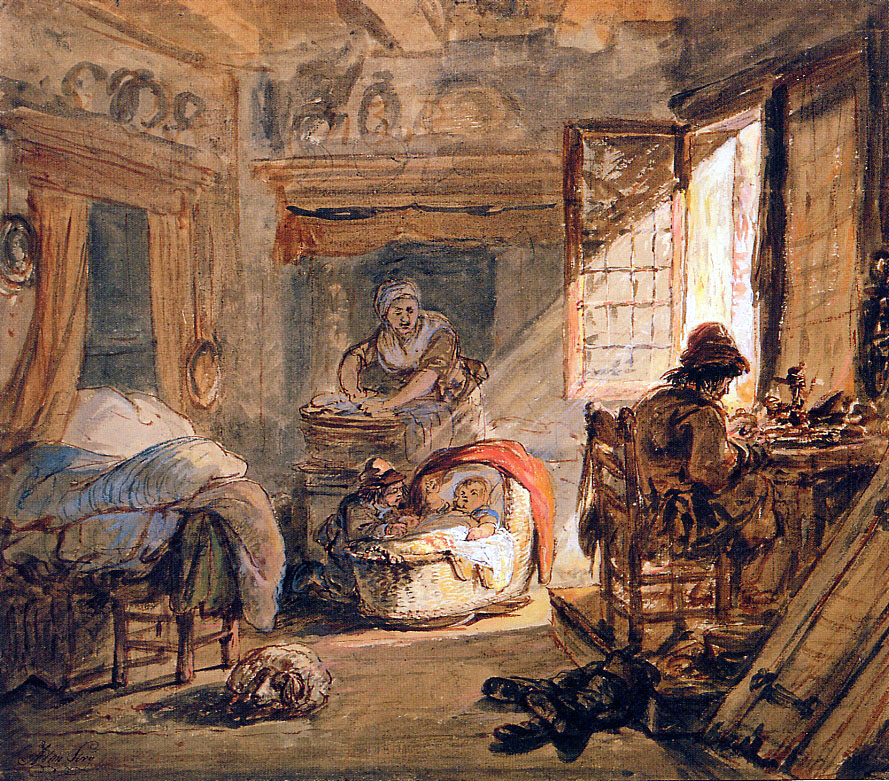
\includegraphics[width=\linewidth]{images/abraham-van-strij_cobbler-and-his-family.jpg}
		\caption{Neoclassicism}
		\label{MLEDdet}
	\end{subfigure}
	\hfil
	\begin{subfigure}{.28\textwidth}
		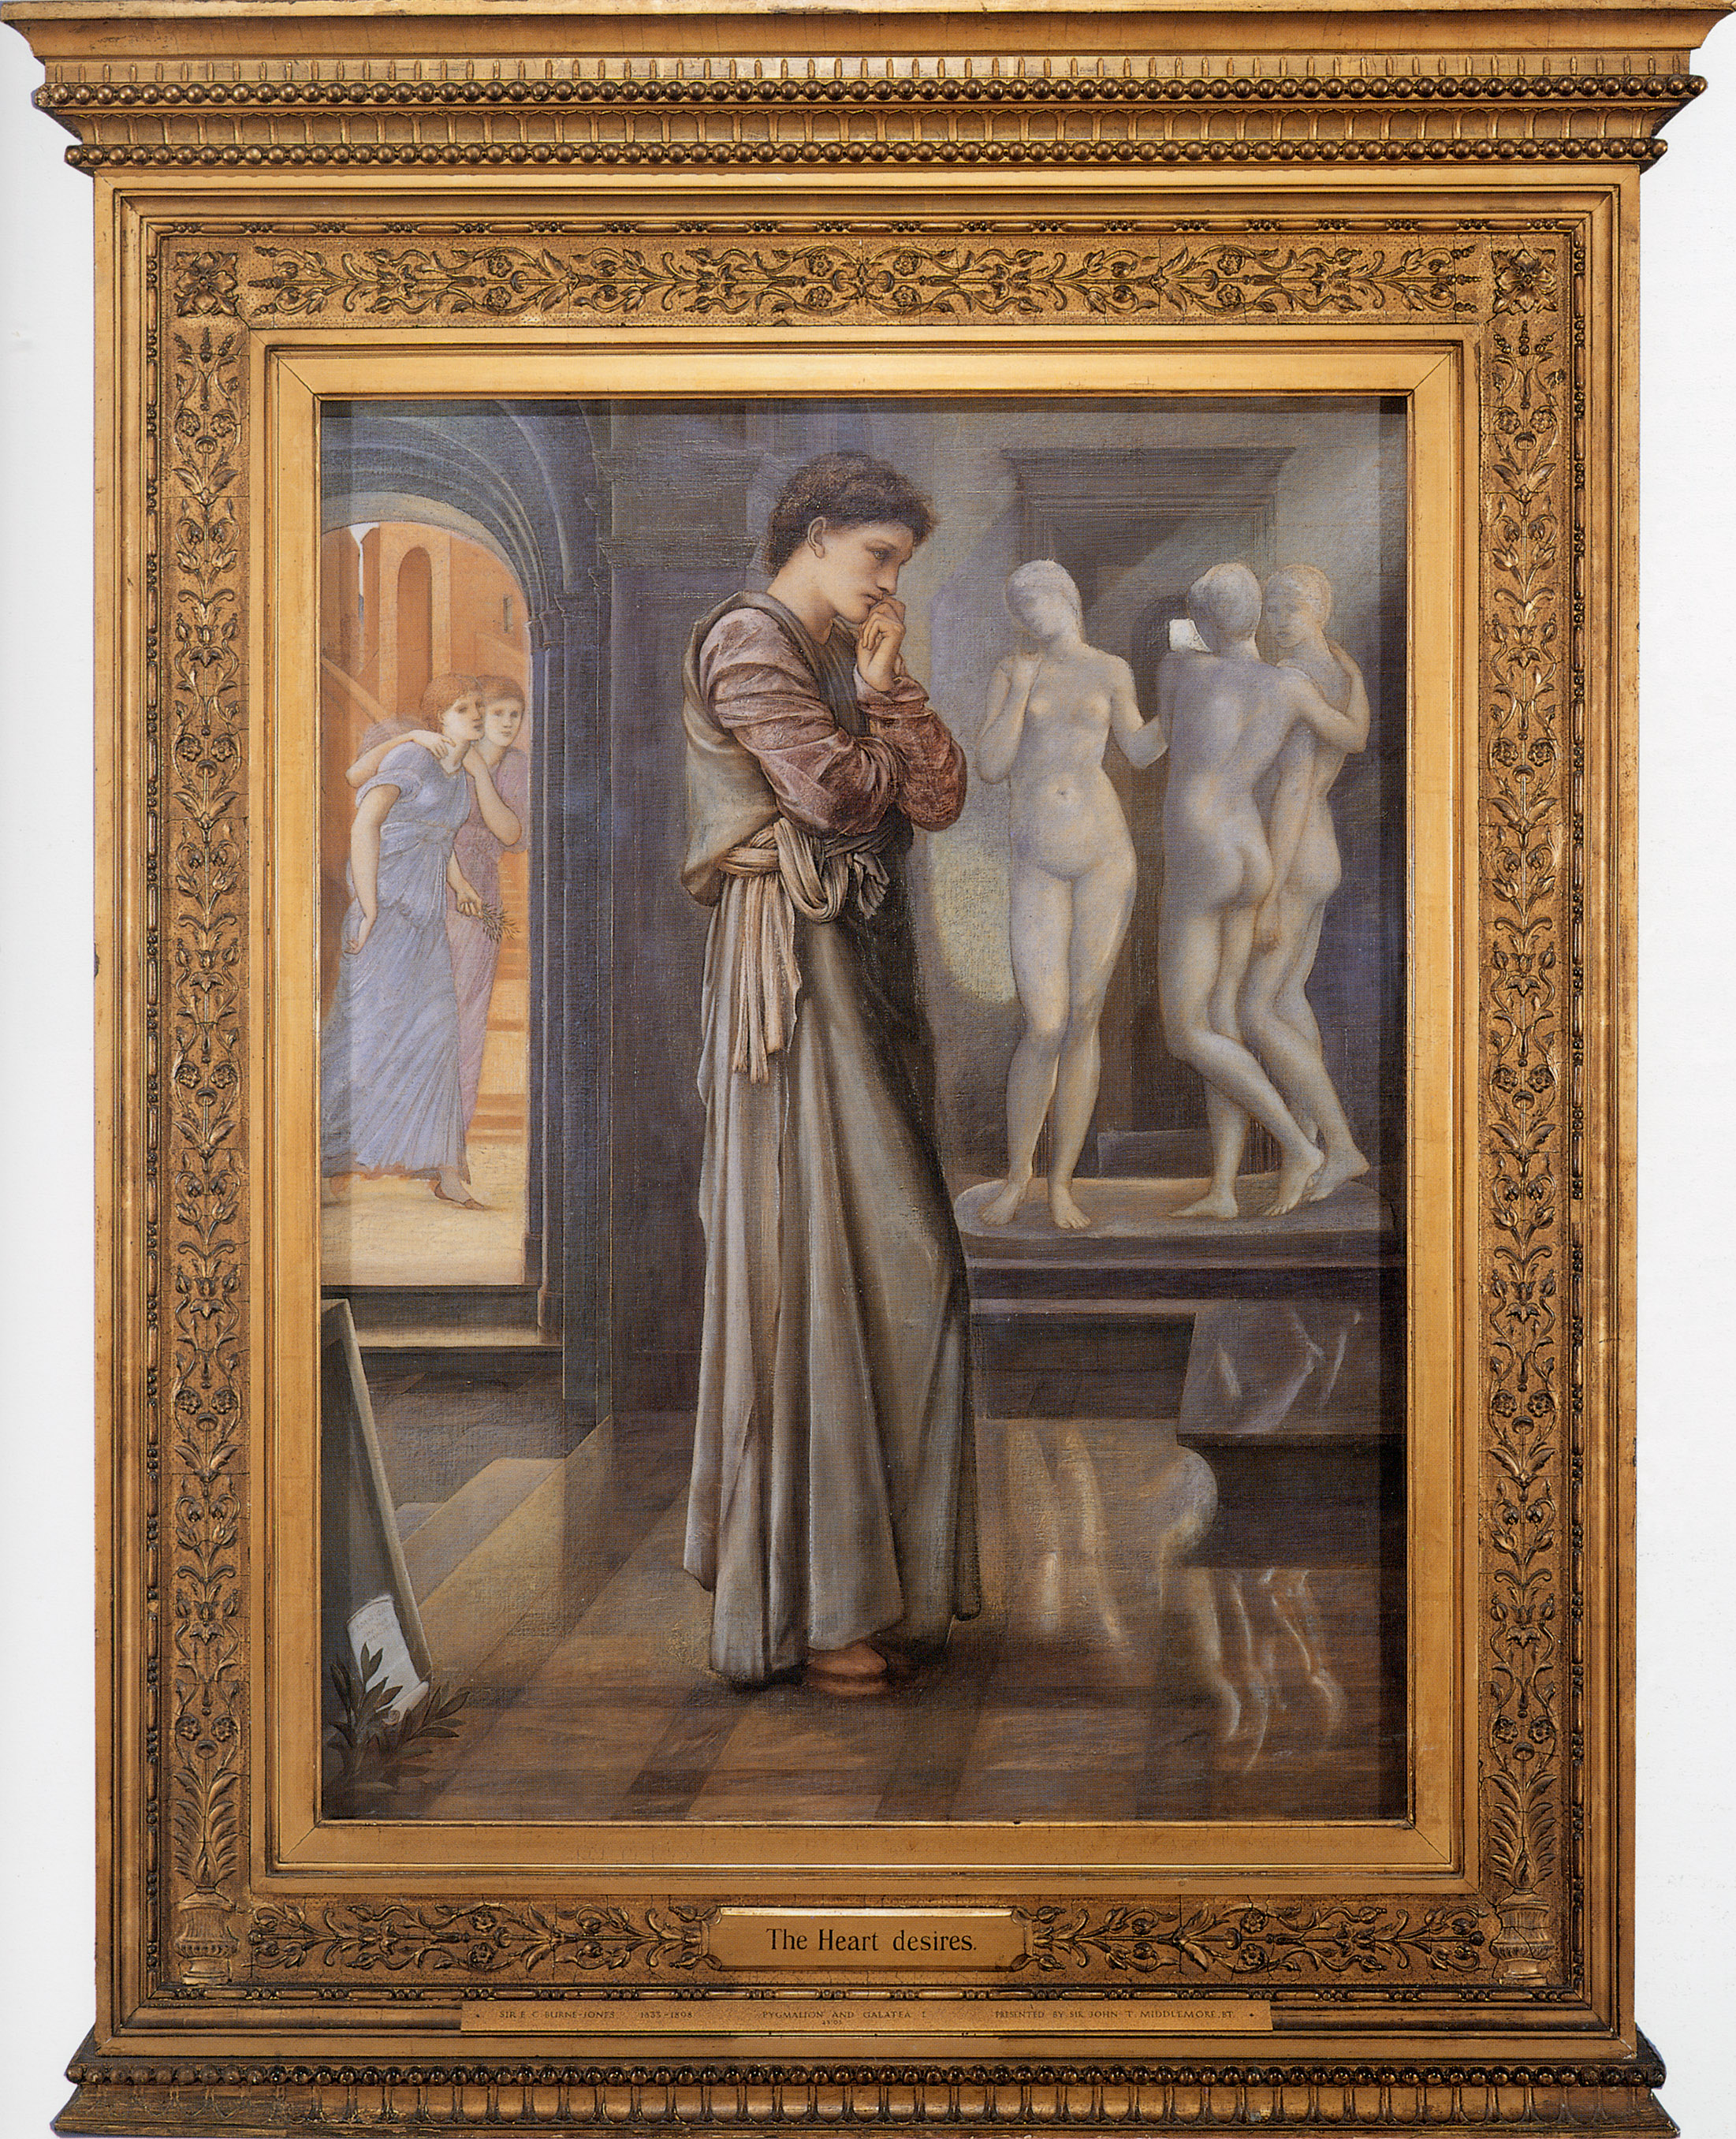
\includegraphics[width=\linewidth]{images/edward-burne-jones_the-heart-desires.jpg}
		\caption{Romantism}
		\label{energydetPSK}
	\end{subfigure}	
	\medskip
	\hfil
	\begin{subfigure}{.36\textwidth}
		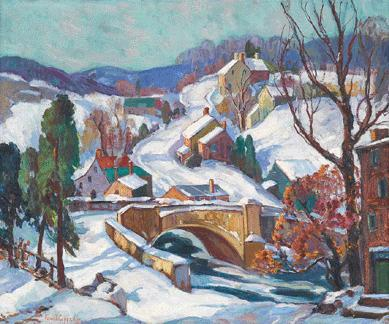
\includegraphics[width=\linewidth]{images/fern-coppedge_january-sunshine.jpg}
		\caption{Impressionism}
		\label{velcomp}
	\end{subfigure}
	\hfil
	\begin{subfigure}{.28\textwidth}
		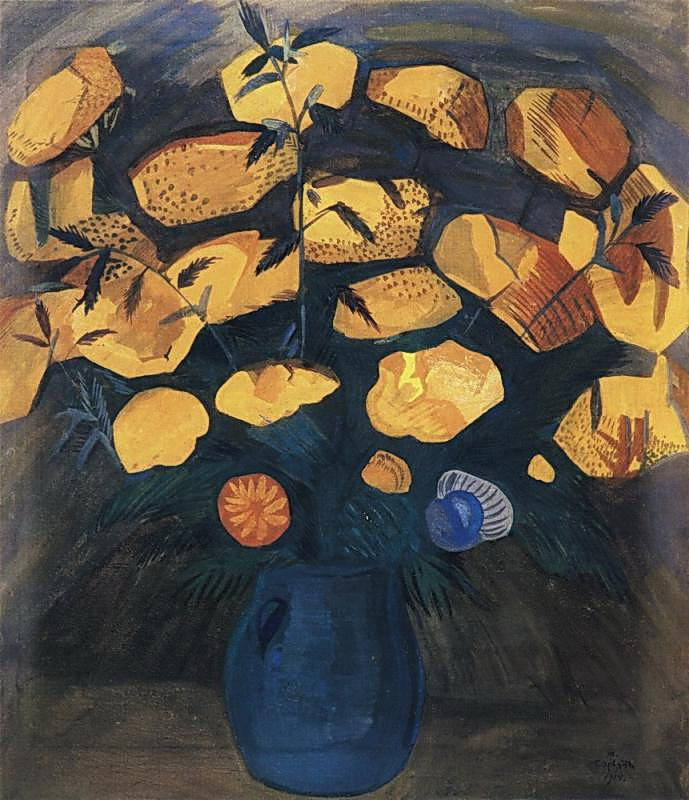
\includegraphics[width=\linewidth]{images/martiros-saryan_yellow-flowers-1914.jpg}
		\caption{Expressionism}
		\label{estcomp}
	\end{subfigure}
	\hfil	
	\caption{Four paintings from the WikiArt dataset with their respective class.}
	\label{fig:wikiart}
\end{figure}

    The architecture of AlexNet consists of convolutional, pooling, and FC layers. Starting with an input layer of 224x224x3 (224x224 dimensions and 3 channels representing the RGB spectrum). The first convolutional layer applies a filter of size 96 with stride, extracting low-level features like as edges and corners. After each of the first two convolutional layers, a max pooling layer with filter and stride is applied, hence reducing spatial dimensions and aiding in capturing invariant features. Local Response Normalization layers are applied between convolutional pooling layers to enhance generalization. The subsequent conv layers employ smaller filters (5x5 and 3x3) to capture more complex patterns and higher-level features. At the deepest level, following the convolutional and pooling layers, three fully connected (FC) layers of 4096 neurons each are present, with the final fully connected layer (output layer) having 1000 neurons (number of classes in the ImageNet dataset) and outputting the respective unnormalised (1000) logits. The softmax activation function computes the probabilities of each class given the input image using the logits acquired previously from the FC layer. An illustration of the AlexNet architecture is shown in Figure \ref{fig:alexnet}. \\
    	
	An important aspect of transfer learning is fine-tuning. In this case, a selection of the final fully connected layers are removed from the pre-trained model and re-trained from scratch. Unfreezing the top layers refers to making those layers trainable so that their weights can be fine-tuned based on the specific task or dataset. As the network begins by extracting generalized low-level features of the data and proceeds to more specific and dependent characteristics as the layers get deeper, this allows the model to keep low-level representations and be re-trained from scratch on the specific features of the dataset, which in practice is smaller and with a more specialized context that the one the pre-trained model has been trained on. \\


	\begin{figure}		
	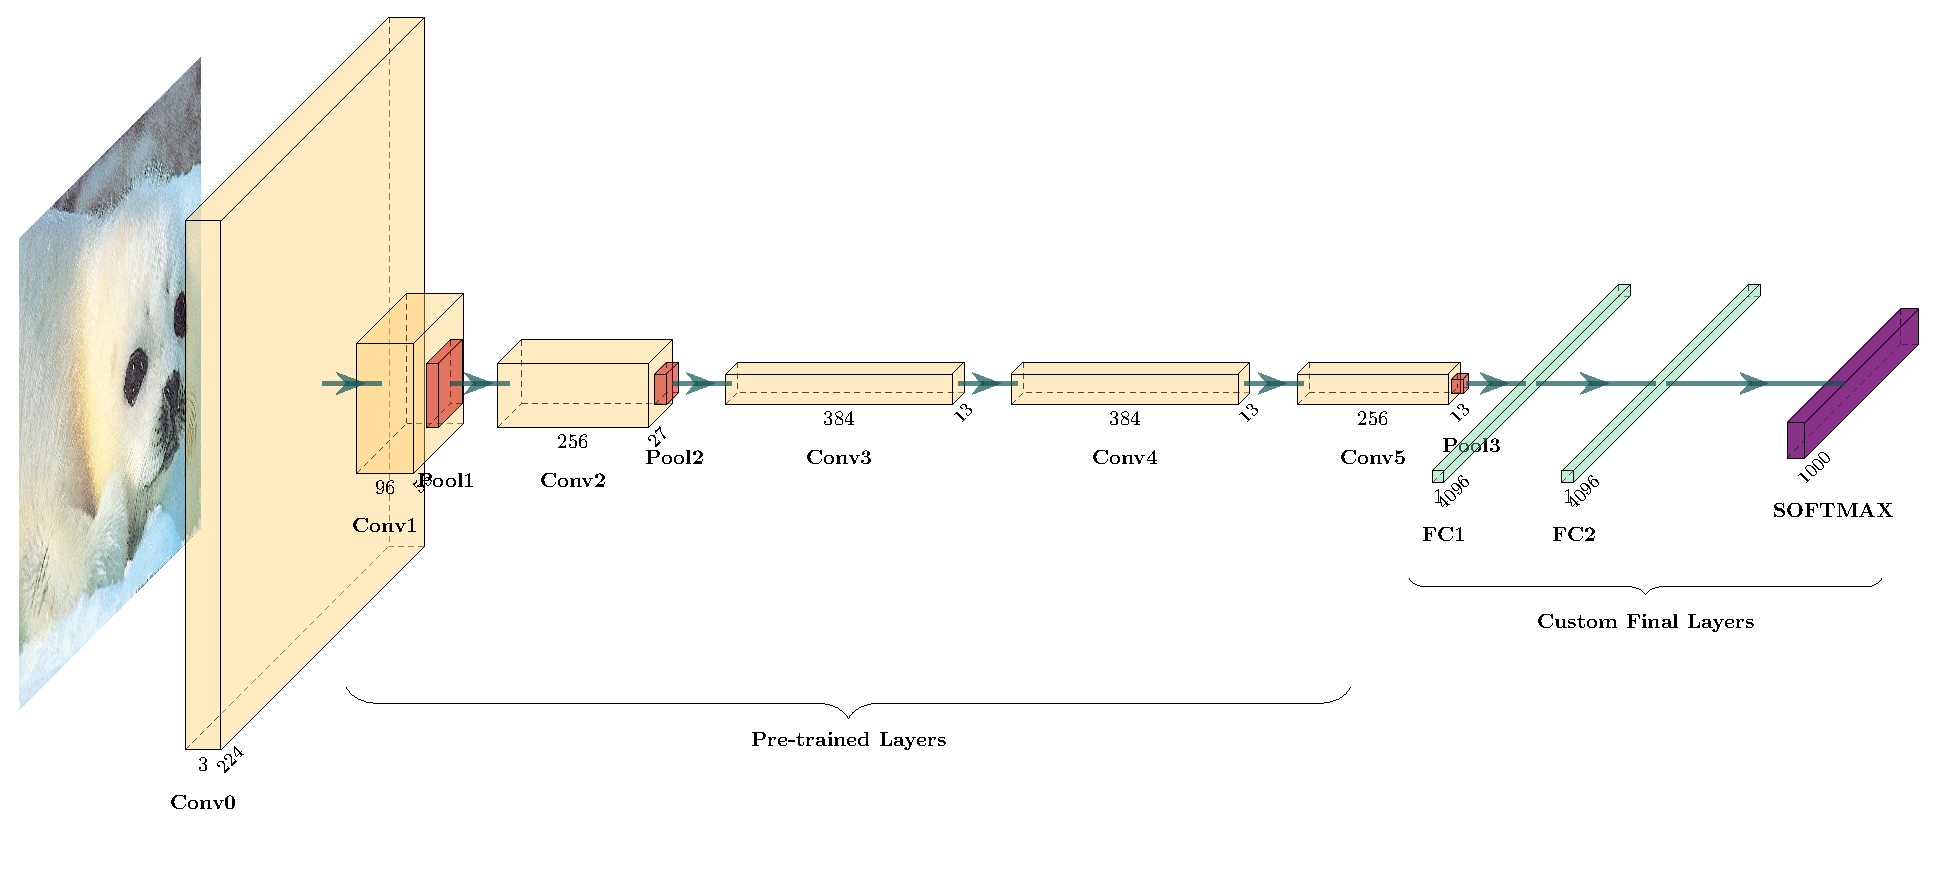
\includegraphics[width=1.0\textwidth]{images/alexnet.pdf}	
	\caption{Illustration of the architecture of AlexNet, a deep convolutional neural network (cNN) proposed by Alex Krizhevsky, Ilya Sutskever, and Geoffrey Hinton in 2012. The architecture of AlexNet gained significant attention and became a breakthrough model in the field of computer vision when it won the ImageNet Large Scale Visual Recognition Challenge (ILSVRC) in 2012, significantly outperforming the state-of-the-art methods of that period. In the task of transfer learning, the final FC layers (denoted with an underbrace and noted \textit{custom final layers}) are re-trained from scratch (fine-tuned) to capture the higher-level features of our feature-specific dataset, while vastly reducing the coputational costs of training a complete cNN architecture from scratch. Note that in our implementation on WikiArt, since we are dealing with 10 classes, the 1000 logits in the final layer are being replaced with 10 logits (\code{num\_classes=10}).}
	\label{fig:alexnet}
	\end{figure}
	
	We begin by automatically obtaining a total of 4000 paintings from WikiArt, using the accompanied script, resulting in a 1.7 GB folder (located at \code{Utilities/data/images}), and split into a training and a validation set (paths of images on the files \code{Utilities/data/train.txt} and \code{Utilities/data/test.txt}), and then obtaining the weights of the pre-trained AlexNet model on ImageNet (\code{Weights/bvlc\_alexnet.npy}). Learning parameters are left as default, that is, \code{learning\_rate = 0.01}, \code{num\_epochs = 10}, \code{batch\_size = 128} and \code{dropout\_rate = 0.5}, \code{num\_classes = 10}. By setting in the \code{train\_layers} list the name of the layers we are interested in un-freezing and re-training (and hence skipping the layers that are not named in the list), we can remove for example the last FC layer (\textit{FC2} in Figure \ref{fig:alexnet}) or the last two FC layers (\textit{FC2} and \textit{FC1} in Figure \ref{fig:alexnet}) and re-training by fine-tuning them. \\
	
	We obtain the defined summaries (cross-entropy loss and accuracy) every \code{display\_step = 3} batches and plot them using Tensorboard\footnote{\url{https://www.tensorflow.org/tensorboard}}. By unfreezing the last fully-connected (FC) layer, a validation accuracy of \code{0.39062} while by unfreezing the two final FC layers a validation accuracy of \code{0.40625}. \\
	
	The training accuracy and cross-entropy loss of each of the two fine-tuning cases mentioned previously are illustrated in Figures \ref{fig:tb1} and \ref{fig:tb2}, while the histogram and distribution of the gradients of the biases and weights of the re-trained FC layers are available in the Appendix. Notice how the plots are a bit smoother when two FC layers are unfreezed and retrained.
	
	\begin{figure}[hbt!]
		\centering
		\hfil
		\begin{subfigure}{.40\textwidth}
			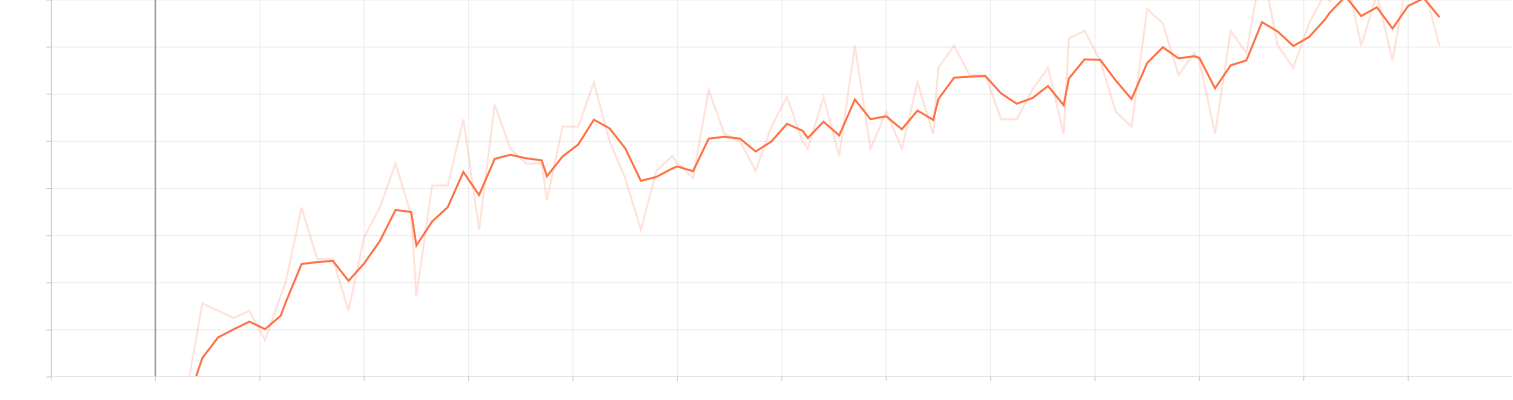
\includegraphics[width=\linewidth]{images/accuracy_fc8.png}
			\caption{Training accuracy}
			\label{MLEDdet}
		\end{subfigure}
		\hfil
		\begin{subfigure}{.40\textwidth}
			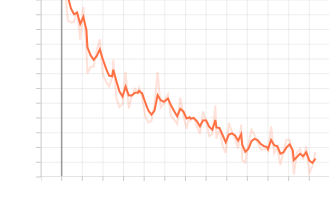
\includegraphics[width=\linewidth]{images/loss_fc8.png}
			\caption{Training cross-entropy loss}
			\label{energydetPSK}
		\end{subfigure}	
	\label{fig:tb1}
	\caption{Training Accuracy and loss on the un-freezed AlexNet with the final FC layer (\code{fc8}) re-trained, using Tensorboard.}
	\end{figure}

	When we remove and retrain the last FC layer of the network, it is probable that the network may struggle adapting to the new task, resulting in a lower accuracy. This happens since the final FC layer maps the learned features to the specific classes of the original ImageNet dataset (two orders of magnitude lower and of different context), which may not directly correspond to the feature representation of the different classes in the WikiArt dataset. This happens because the earlier layers in a deep neural network, like the convolutional layers, are responsible for learning general features, while the later FC layers tend to capture more specific and task-dependent information of the data.
	\\
	
	Similarly, when the last two FC layers are un-freezed and re-trained, although the network learns and adapts the richer high-level feature representations of WikiArt more extensively, this results in a slight improvement in accuracy, although not enough to fully capture the differences between different style images in the unknown test set. Of course, this stems from the degree of similarity between Imagenet and the target dataset (in our case, WikiArt). \\
	
	In more detail, a poor performance of the pre-trained AlexNet on WikiArt can be explained further by the following points: \\
	
	\begin{enumerate}[I]
		\item \textit{Textures \& colors}: Paintings differ than natural images due to their textures that are dependent on the painting technique used, the material of the brushes, the stroke, the personal style of the painter, the color palette used etc. These combinations can significantly vary between different art movements and styles, thus making the pre-trained AlexNet less effective in capturing these artistic characteristics.
		
		\item \textit{Semantic Meaning}: Paintings are created to convey various artistic concepts, emotions, and narratives, which might not align with the object-centric semantics learned by AlexNet from ImageNet. The pre-trained model may not have learned the specific visual cues and symbolic representations relevant to the artistic concepts present in the WikiArt dataset.
		
		\item \textit{Classes}: The ImageNet dataset consists of various categories including a plethora of species and breeds of animals (250: siberian husky, 265: toy puddle etc), items (514: cowboy boot, 530: dining clock, 849: teapot etc) and vehicles (561: forklift, 751: race car, 864: tow car etc). On the other hand, paintings in the WikiArt dataset are focused on specific art movements, genres, or themes, hence the pre-trained AlexNet might not have learned discriminative features for these specific painting-related themes.
	\end{enumerate}

   	\begin{figure}[hbt!]
   		\centering
    	\hfil
    	\begin{subfigure}{.40\textwidth}
    		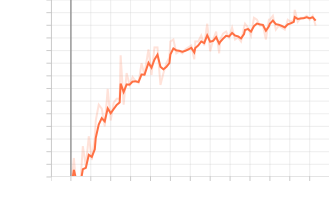
\includegraphics[width=\linewidth]{images/accuracy_fc7_fc8.png}
    		\caption{Training accuracy}
    		\label{MLEDdet}
    	\end{subfigure}
    	\hfil
    	\begin{subfigure}{.40\textwidth}
    		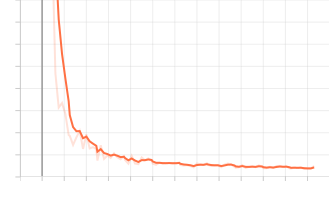
\includegraphics[width=\linewidth]{images/loss_fc7_fc8.png}
    		\caption{Training cross-entropy loss}
    		\label{energydetPSK}
    	\end{subfigure}	
        \label{fig:tb2}
    	\caption{Training Accuracy and loss on the un-freezed AlexNet with the final two FC layers (\code{fc7}, \code{fc8}) re-trained, using Tensorboard.}
    \end{figure}

    \pagebreak
    
    \subsection{Assignment 3b}
    
    For part B, the task is to visualize the saliency map of various input images, using the VGG16 architecture and the Vanilla Gradient method. \\
    
     
    \begin{figure}[h]
    	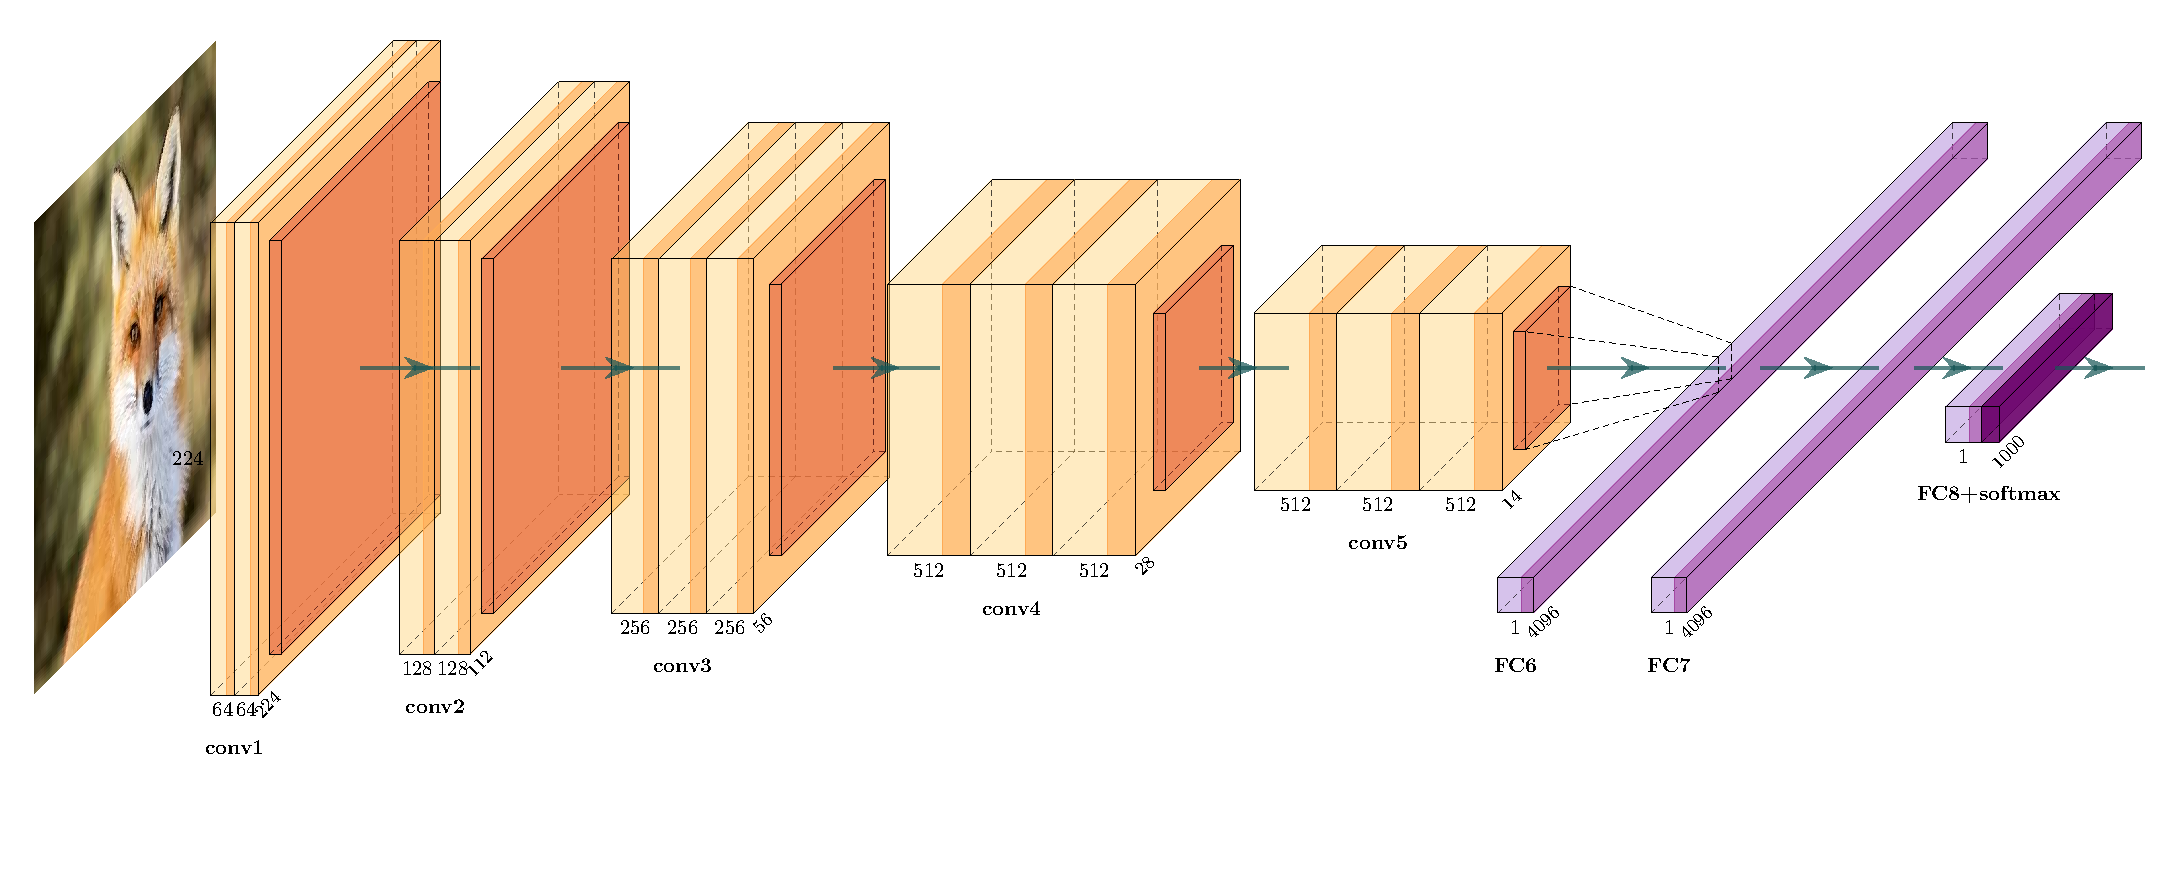
\includegraphics[width=1.0\textwidth]{images/vgg16.pdf}
    	\caption{Illustration of the architecture of VGG16. Like before, \textit{redfox} corresponds to class 277 in ImageNet.}
    	\label{fig:VGG16}
    \end{figure}

    VGG16 (Visual Geometry Group 16) is a convolutional neural network (CNN) architecture developed by the Visual Geometry Group at the University of Oxford\footnote{Simonyan, K., \& Zisserman, A. (2014). \textit{Very Deep Convolutional Networks for Large-Scale Image Recognition}. arXiv preprint arXiv:1409.1556.}, that gained significant attention for its impressive performance in the 2014 ILSVRC challenge. Trained on a subset of ImageNet with 1000 classes, similarly to AlexNet, as the name suggests, VGG16 is comprised of 16 layers (13 convolutional layers and 3 fully connected layers). \\
    
    The architecture utilizes 3x3 convolutional filters consistently throughout the network as well as implementing max-pooling layers and finally a softmax activation function, like AlexNet. See Figure \ref{fig:VGG16} for an illustration of the architecture of the model. \\
    
    \begin{figure}[hbt!]
    	\centering
    	\hfil
    	\begin{subfigure}{.34\textwidth}
    		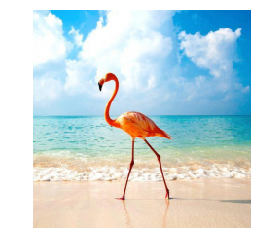
\includegraphics[width=\linewidth]{images/flamingo.png}
    		\caption*{Image of a flamingo by the beach}
    		\label{MLEDdet}
    	\end{subfigure}
    	\hfil
    	\begin{subfigure}{.34\textwidth}
    		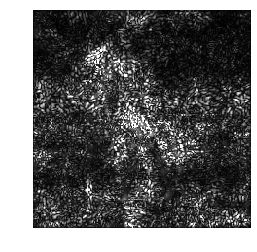
\includegraphics[width=\linewidth]{images/flamingo_saliency.png}
    		\caption*{Saliency map of the flamingo}
    		\label{energydetPSK}
    	\end{subfigure}
        \hfil
        \label{fig:flamingo}
        \caption{Input image of a flamingo, classified by VGG16 in class 130 (class flamingo) with its vanilla gradient saliency map.}
    \end{figure} 
    
    The purpose of \textit{saliency maps} is to serve as a visualization technique, offering valuable understanding into the specific reasoning behind a deep learning model's decision (what the model "sees") on the classification of an image. Saliency maps are rendered as heatmaps of the original image, where intense colors represent regions that have a big impact on the model's decision and are more attention-grabbing than the remaining parts of the image. It allows us to obtain a behind-the-curtain understanding on what high-level features of the input influence the final classification decision but also to distinguish which features lead to incorrect decisions\footnote{YouTube. (2021). L13.8 \textit{What a CNN Can See - STAT 453: Intro to Deep Learning and Generative Models}, University of Wisconsin-Madison. Available on YouTube. Retrieved May 12, 2023, from \url{https://www.youtube.com/watch?v=PRFP5YC3u7g}.}. \\
    
    We create the saliency map, first of the flamingo and then of the three images in the \code{MyImages} folder, after classifying them on the VGG16 network, using the original saliency map algorithm in supervised deep learning introduced by Simonyan et. al. in 2013\footnote{Karen Simonyan, Andrea Vedaldi, and Andrew Zisserman, \textit{Deep Inside Convolutional Networks: Visualising Image Classification Models and Saliency Maps}, ICLR Workshop 2014.}, known as \textit{Vanilla Gradient Mask} \footnote{\url{https://andrewschrbr.medium.com/saliency-maps-for-deep-learning-part-1-vanilla-gradient-1d0665de3284}}. Vanilla Gradient has proven to be quite robust compared to other techniques, while also standing out as the simplest algorithm among gradient-based approaches. The calculation and visualization of the vanilla gradient is the following:
    
    \begin{enumerate}
    	\item Do a forward pass of the image $I$ through the network
    	\item Calculate the scores for every class $C$, $S_C (I) = w^T_C I + b_c$
    	\item Enforce the derivative w.r.t. $I$ (i.e. the input image) of score vector $S$ at last layer for all classes except class $C$ to be $0$, while for $C$ set it to $1$, $\displaystyle \text{argmax}_I S_C(I) - \lambda ||I||^2_2$
    	\item Back-propagate this derivative until the start, $w = \frac{\partial S_C}{\partial I} |_{I_0}$
    	\item Render the gradients and obtain the saliency map of $I$
    \end{enumerate}

    We implement the above steps in the accompanied \code{.ipynb} notebook of the report and firstly obtain the saliency map of the flamingo, shown in Figure \ref{fig:flamingo}. \\
    
    The high values around the body of the flamingo in the saliency map can be explained by the body of the flamingo being vibrant in color (pink due to their food, algae and brine shrimp) and thus highly distinct from its surroundings. High values around the clouds can be attributed to the high contrasting color between the flamingo and the sky, as well as the environment in which an image of a flamingo is often captured. \\
    
    We then repeat the process for the rest of the images located in the folder \code{My-Images}, a doberman (class 236), a teddy bear (class 850) and an image of a cat (class 281). The resulting saliency maps for each of the three images in the aforementioned folder are shown in Figure \ref{fig:myImages}, after being classified correctly by the model. Some explaining on the resulted saliency maps for the three images is the following:
    
    \begin{itemize}
    	\item \textit{Dog:} The highlighting of the crossed legs and all-around shape suggests that they provide cues about the dog's posture and movement. The highlighting of the face, the nose-mouth region and the ears, are a crucial area for attention as it predominately characterizes the dog species.
    	
    	\item \textit{Teddy bear:} Similarly to the dog, the high values around the top of the head and legs in the saliency map of the teddy bear are a result of its distinct shape and the presence of prominent features in teddy bears. The legs might also be considered visually significant as they provide information about the pose or position of the teddy bear (different than a wild bear).
    	
    	\item \textit{Cat:} Finally, the areas around the nose, eyes, ears exhibit distinct shapes and patterns present in cats (and big cats in general like leopards), with cats being differentiated from other big cats due to their smaller shape and stature, thus causing the saliency map to depict attention on the all-around shape of the cat.
    	
    \end{itemize}
    
    \begin{figure}[hbt!]
    	\centering
    	\hfil
    	\begin{subfigure}{.34\textwidth}
    		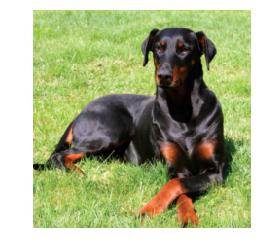
\includegraphics[width=\linewidth]{images/doberman.png}
    		\caption{Doberman}
    		\label{MLEDdet}
    	\end{subfigure}
    	\hfil
    	\begin{subfigure}{.34\textwidth}
    		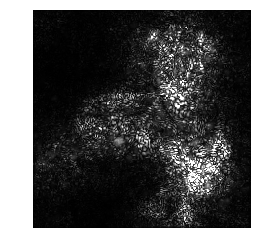
\includegraphics[width=\linewidth]{images/doberman_saliency.png}
    		\caption*{Corresponding saliency map}
    		\label{energydetPSK}
    	\end{subfigure}	
    	\medskip
    	\hfil
    	\begin{subfigure}{.33\textwidth}
    		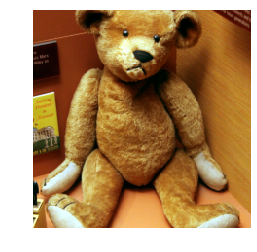
\includegraphics[width=\linewidth]{images/teddy_bear.png}
    		\caption{Teddy Bear}
    		\label{velcomp}
    	\end{subfigure}
    	\hfil
    	\begin{subfigure}{.33\textwidth}
    		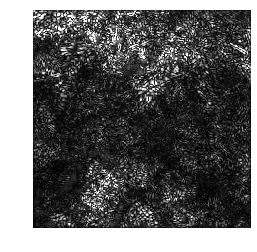
\includegraphics[width=\linewidth]{images/teddy_bear_saliency.png}
    		\caption*{Corresponding saliency map}
    		\label{estcomp}
    	\end{subfigure}	
    	\medskip
    	\hfil
    	 \begin{subfigure}{.33\textwidth}
    		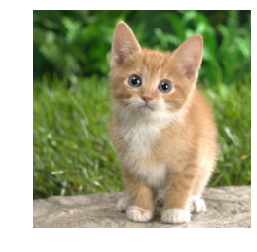
\includegraphics[width=\linewidth]{images/cat.png}
    		\caption{Cat}
    		\label{velcomp}
    	\end{subfigure}
    	\hfil
    	\begin{subfigure}{.33\textwidth}
    		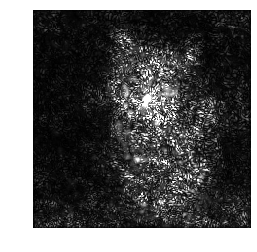
\includegraphics[width=\linewidth]{images/cat_saliency.png}
    		\caption*{Corresponding saliency map}
    		\label{estcomp}
    	\end{subfigure}
    	\hfil	
    	\caption{The three images in the \code{myImages} folder with their respective vanilla gradient saliency maps.}
    	\label{fig:myImages}
    \end{figure}

\pagebreak

\begin{thebibliography}{4}
	\bibitem{goodfellow2016} Goodfellow, I., Bengio, Y., \& Courville, A. (2016). \textit{Deep learning}. MIT Press.
\end{thebibliography}

\pagebreak

\appendix

\section{Appendix}

\subsection{Troubleshooting}

The \code{.ipynb} notebooks of the assignment were run on \textbf{Ubuntu 22.04 LTS}, in \textbf{Python 3.5.6} (|Anaconda, Inc.| (default, Aug 26 2018, 21:41:56) [GCC 7.3.0] linux /home/nikolas/anaconda3/envs/cs587\_hw3/bin/python), downgraded \textbf{NumPy 1.16.5} (['/home/nikolas/anaconda3/envs/cs587\_hw3/lib/python3.5/site-packages/numpy'] and scikit-learn.
1.16.5), \textbf{TensorFlow 1.15}, \textbf{Pandas} and \textbf{Pickle 4.0.0} in the created \code{cs587\_hw3} Anaconda virtual environment (\code{conda create cs587\_hw3 python=3.5} and \code{conda activate cs587\_hw3)}. Monitoring of the model was done using Tensorboard, \code{tensorboard --logdir finetune\_alexnet/wikiart}. The source files of both \code{AlexNet.py} and \code{VGG16.py} containing the \code{np.load} command were modified to include the \code{allow\_pickle=True} argument. \\

 One can obtain the list of packages we had to downgrade and install while trying to get the assignment running, by executing \code{pip list --format=freeze > requirements.txt} in the \code{cs587\_hw3} virtual environment:

\begin{lstlisting}[]
	absl-py==0.15.0
	asn1crypto==1.4.0
	astor==0.8.1
	bleach==3.3.1
	certifi==2020.6.20
	cffi==1.11.5
	colorama==0.4.4
	cryptography==2.3.1
	cycler==0.10.0
	decorator==5.1.1
	defusedxml==0.7.1
	entrypoints==0.2.3
	gast==0.2.2
	google-pasta==0.2.0
	grpcio==1.41.1
	h5py==2.10.0
	idna==3.3
	imageio==2.9.0
	importlib-metadata==2.1.3
	importlib-resources==3.2.1
	ipykernel==4.10.0
	ipython==5.8.0
	ipython-genutils==0.2.0
	ipywidgets==7.4.1
	Jinja2==2.11.3
	jsonschema==2.6.0
	jupyter==1.0.0
	jupyter-client==5.3.3
	jupyter-console==5.2.0
	jupyter-core==4.5.0
	Keras-Applications==1.0.8
	Keras-Preprocessing==1.1.2
	kiwisolver==1.1.0
	Markdown==3.2.2
	MarkupSafe==1.0
	matplotlib==3.0.3
	mistune==0.8.3
	nbconvert==5.5.0
	nbformat==5.1.3
	networkx==2.4
	notebook==5.5.0
	numpy==1.16.5
	olefile==0.46
	opt-einsum==3.3.0
	packaging==20.9
	pandas==0.23.4
	pandocfilters==1.5.0
	pexpect==4.8.0
	pickleshare==0.7.5
	Pillow==4.0.0
	pip==20.3.4
	prompt-toolkit==1.0.15
	protobuf==3.19.6
	ptyprocess==0.7.0
	pycparser==2.20
	Pygments==2.11.2
	pyOpenSSL==18.0.0
	pyparsing==2.4.7
	PySocks==1.6.8
	python-dateutil==2.8.2
	pytz==2021.3
	PyWavelets==1.1.1
	pyzmq==17.1.2
	qtconsole==4.7.7
	QtPy==1.11.2
	scikit-image==0.15.0
	scipy==1.4.1
	Send2Trash==1.8.0
\end{lstlisting}
 
\pagebreak

\subsection{Extra figures}

%\begin{figure}[hbt!]
%	\centering
%		\includegraphics[width=\linewidth]{images/computational_graph_fc8.png}
%		\caption{Computational Graph of AlexNet, with the final FC layer un-freezed and re-trained on WikiArt using Stochastic Gradient Descent.}
%\end{figure}

%    \begin{figure}[hbt!]
%	\centering
%	\includegraphics[width=\linewidth]{images/computational_graph_fc7_fc8.png}
%	\caption*{Computational Graph of AlexNet, with the final two FC layers un-freezed and re-trained on WikiArt using Stochastic Gradient Descent.}
%\end{figure}

%\pagebreak

\begin{figure}[h]
	\centering
	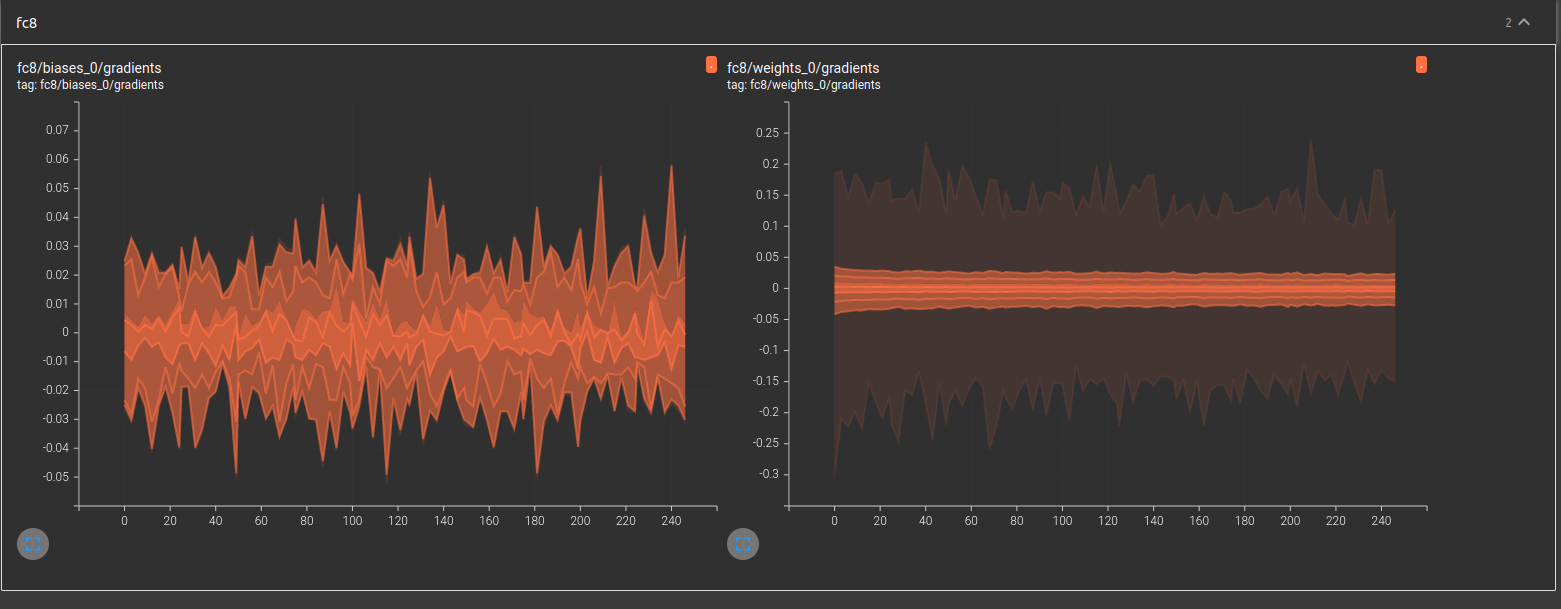
\includegraphics[width=0.85\linewidth]{images/distributions_fc8.png}
	\caption{Gradients distribution for the biases and weights of layer FC8 of the AlexNet model with the final FC layer (fc8) removed and re-trained on WikiArt.}
\end{figure}

\begin{figure}[h]
	\centering
	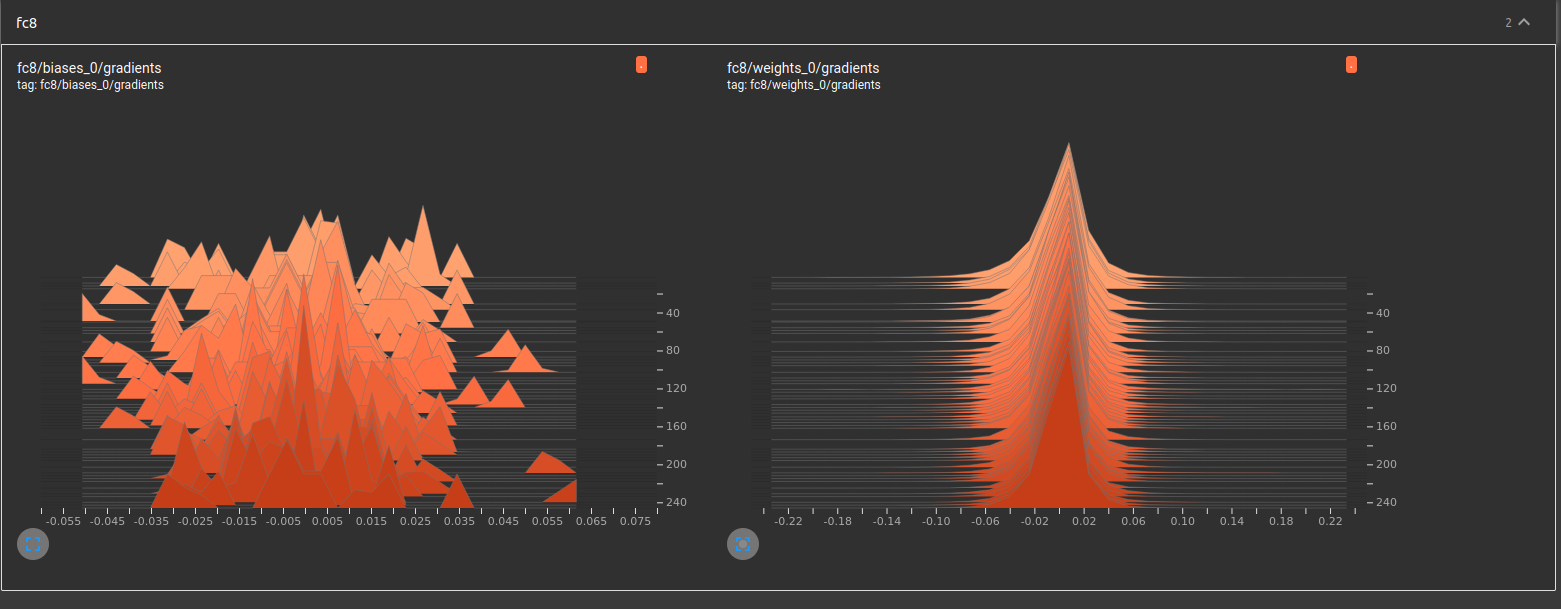
\includegraphics[width=0.85\linewidth]{images/histogram_fc8.png}
	\caption{Histogram for the gradients of the biases and weights of layer FC8 of the AlexNet model with the final FC layer (fc8) removed and re-trained on WikiArt.}
\end{figure}

\begin{figure}[h]
	\centering
	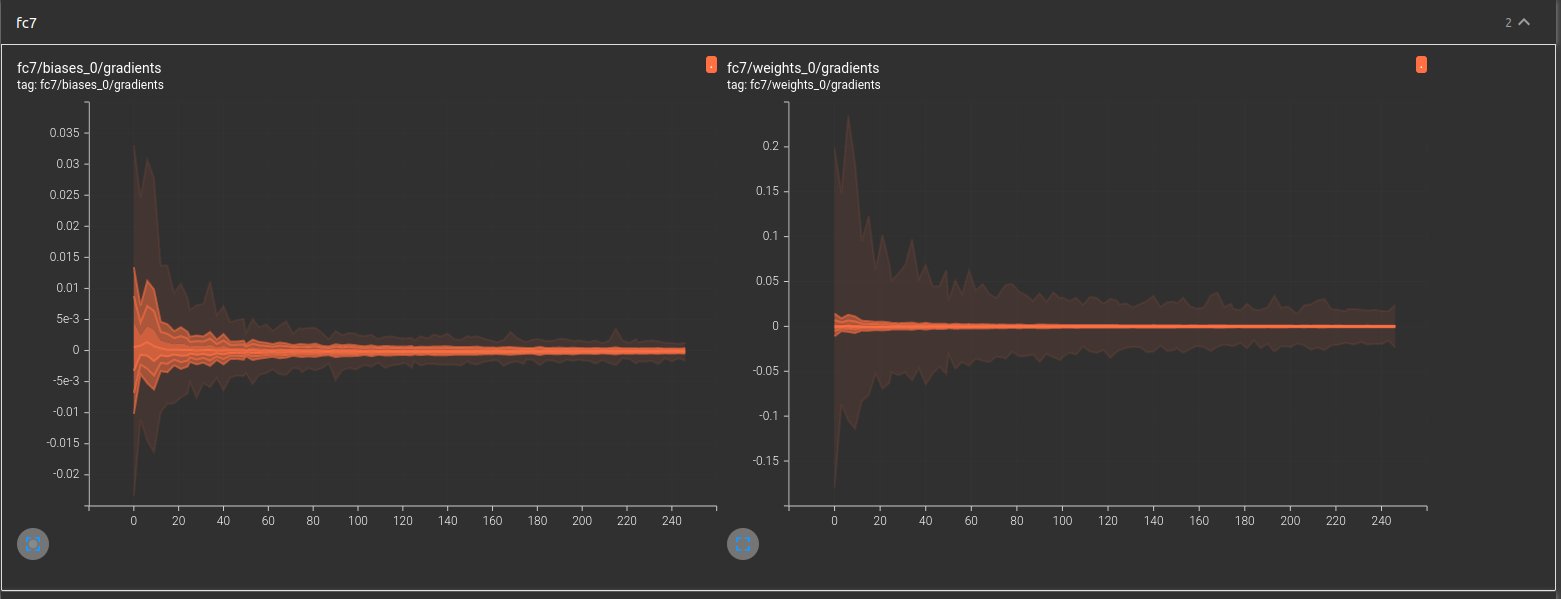
\includegraphics[width=\linewidth]{images/distributions_fc7_2.png}
	\caption{Gradients distribution for the biases and weights of the FC layer \code{fc7} of the AlexNet model with the final two FC layers (\code{fc7} and \code{fc8}) removed and re-trained on WikiArt.}
\end{figure}

\begin{figure}[h]
	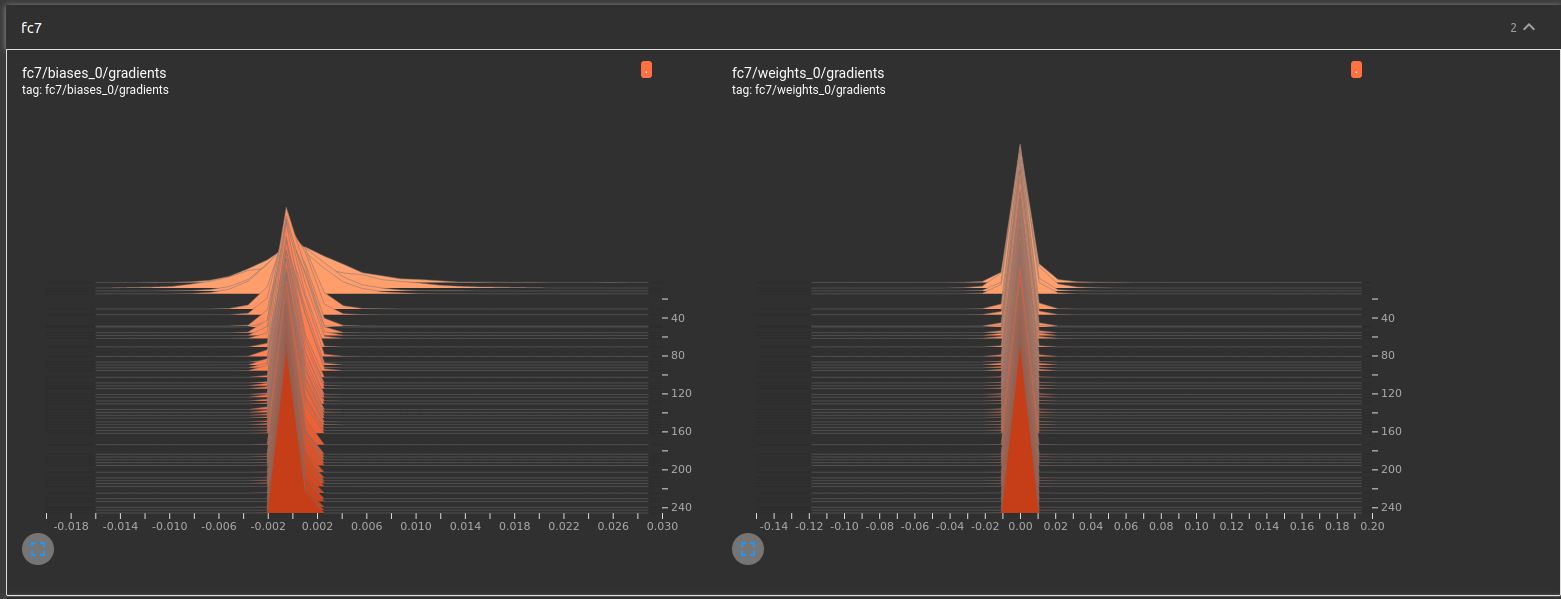
\includegraphics[width=\linewidth]{images/histogram_fc7_2.png} 
	\caption{Histogram for the gradients of the biases and weights of the FC layer \code{fc7} of the AlexNet model with the final two FC layers (\code{fc7} and \code{fc8}) removed and re-trained on WikiArt.}
\end{figure}

\begin{figure}[h]
	\centering
	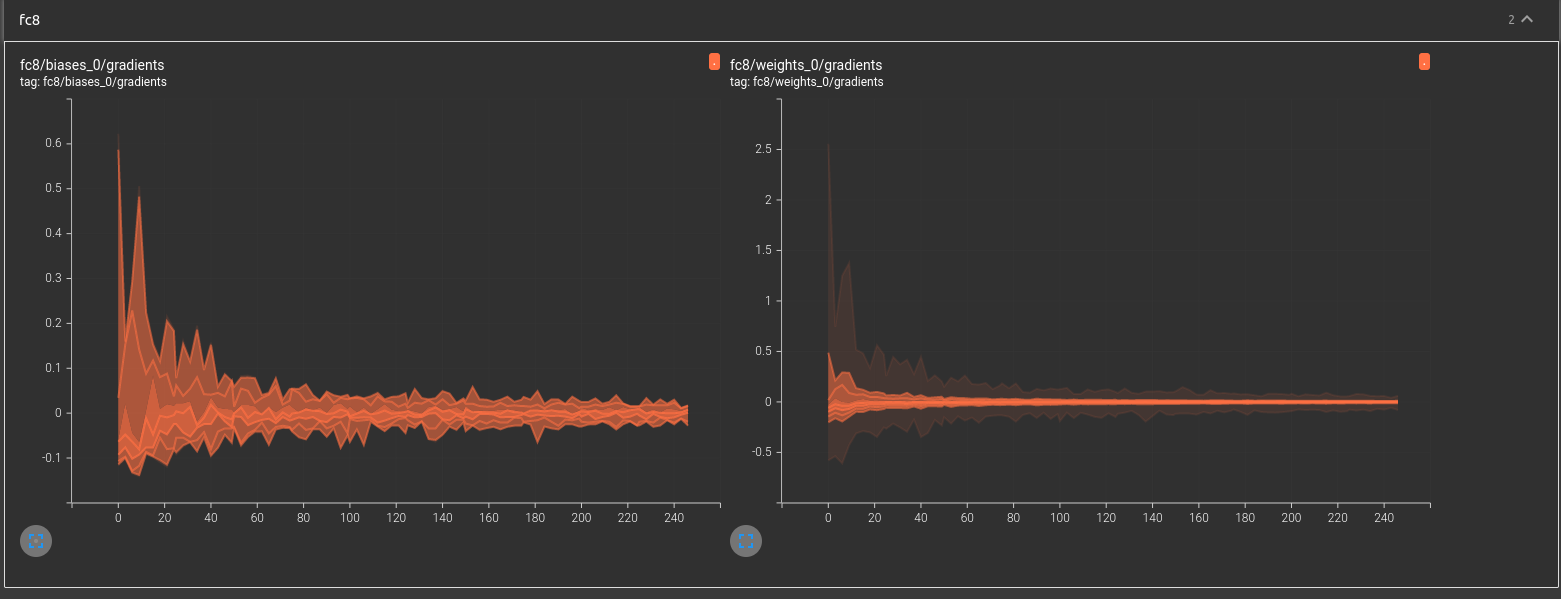
\includegraphics[width=\linewidth]{images/distributions_fc8_2.png}
     \caption{Gradients distribution for the biases and weights of the FC layer \code{fc8} of the AlexNet model with the final two FC layers (\code{fc7} and \code{fc8}) removed and re-trained on WikiArt.}
\end{figure}

\begin{figure}[h]
		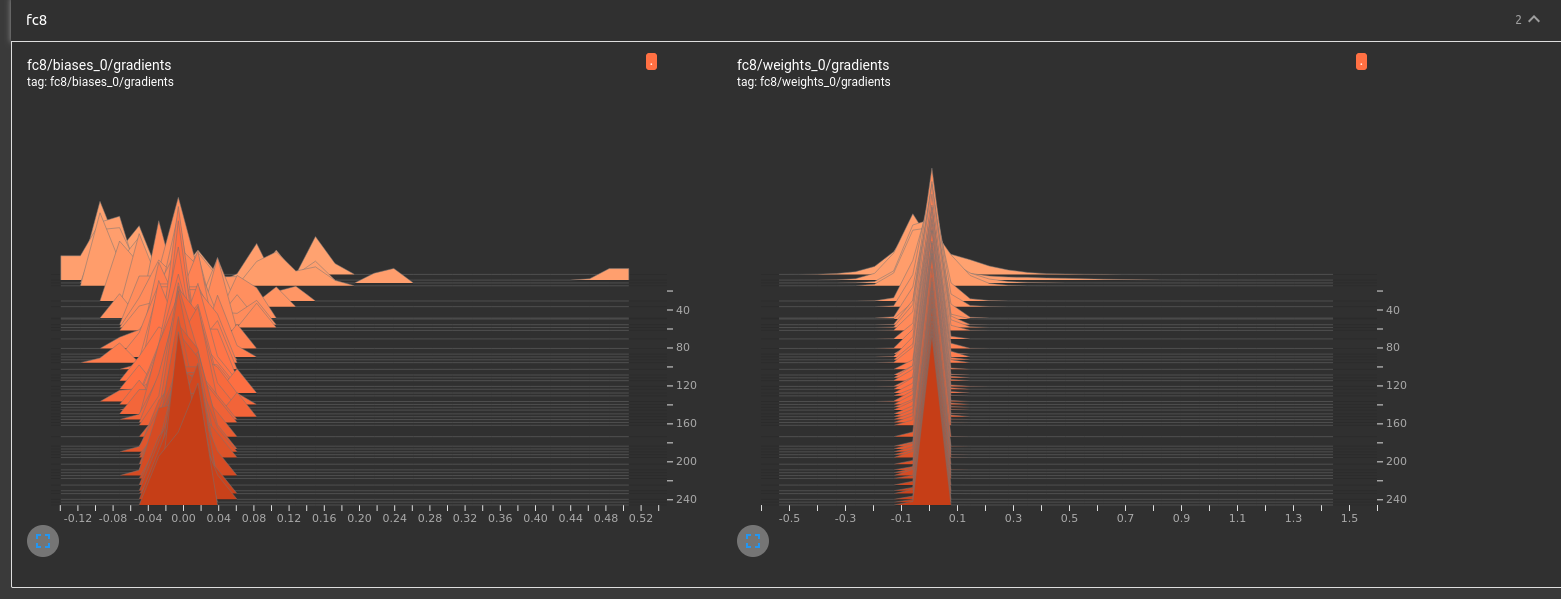
\includegraphics[width=\linewidth]{images/histogram_fc8_2.png} 
		\caption{Histogram for the gradients of the biases and weights of the FC layer \code{fc8} of the AlexNet model with the final two FC layers (\code{fc7} and \code{fc8}) removed and re-trained on WikiArt.}
\end{figure}	


\end{document}
